\section{Segurança, Privacidade e Legislação}
Atualmente, há uma crescente no número de usuários utilizando dispositivos conectados a \textit{Internet}, o que, por um lado mostra que essa tecnologia tão importante está sendo difundida a todas as camadas sociais, mas por outro, gera preocupação quanto as implicações do uso inadvertido das redes.
Nesse contexto, tornou-se comum pessoas mal intencionadas que usam da ignorância de alguns para cometer ataques digitais, prejudicando ou tomando vantagem de pessoas, grupos ou organizações. A afirmativa anterior é confirmada por um gráfico (Figura \ref{fig:cibercrimes}) elaborado pela \emph{Surfshark} \cite{Surfshark}, empresa provedora de serviços de \gls{vpn}, que analisa o crescimento anual de custos em cibersegurança. 
\begin{figure}[h]
	\centering
	\caption{Crescimento anual de custos com cibercrime}
	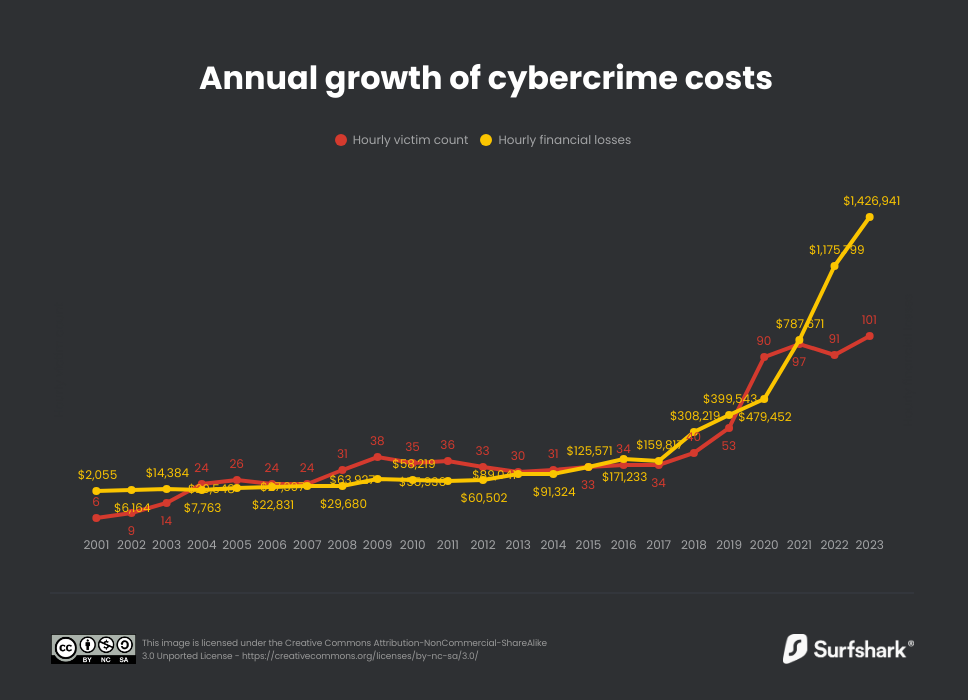
\includegraphics[width=1\textwidth]{cap04-desenvolvimento/images/4-6-annual-growth-of-cybercrime-costs.png}
	\fonte{\cite{Surfshark}}
	\label{fig:cibercrimes}
\end{figure}

Por isso surgiram leis e normas que regularizam como os dados devem ser tratados e também tecnologias que auxiliam a proteger os dois lados da comunicação: os clientes, que desejam ter seus dados protegidos, e das organizações, que precisam se certificar da identidade do usuário.
Isto posto, serão abordadas as técnicas e metodologias adotadas a fim de garantir que o software desenvolvido atenda as demandas da legislação e promova segurança e privacidade a seus utilizadores.

\subsection{Critérios de Segurança e Privacidade}
Na aplicação desenvolvida, foram definidas formas de manter a segurança de todas as partes envolvidas. Foi implementado um método de cadastro e \textit{login} facilitado com geração de \textit{tokens} e também uma infraestrutura de rede que protege o dispositivo que armazena o banco de dados da aplicação.

\subsubsection{Cadastro e \emph{Login} com Conta Google}
Um dos requisitos da entidade parceira, era o desenvolvimento de um sistema de cadastro e \emph{login} facilitados, haja vista que muitos dos clientes tinham dificuldade em acessar a aplicação anterior por constantemente esquecerem sua credenciais (\emph{e-mail} e senha).
Considerando essa dificuldade, foi implementado um sistema de registro e \emph{login} utilizando a \gls{api} de autenticação \emph{OAuth} da Google, pelo fato da maioria dos dispositivos no Brasil apresentarem sistema operacional Android, conforme destaca uma pesquisa \cite{app-my-site}, que geralmente requerem uma conta Google para seu funcionamento. E mesmo indivíduos com aparelhos de outro sistema operacional, comumente possuem contas Google para usufruir de seus serviços.
Assim sendo, a responsabilidade de identificar os usuários da aplicação foi terceirizada para a Google, e quando estes se cadastram, devem aceitar suas políticas e termos de usuário que definem extensamente como os dados são processados, tratados e protegidos.

\subsubsection{Infraestrutura de Rede}
Os dispositivos (máquinas virtuais) que sustentam a aplicação estão hospedados na \gls{aws}, logo sendo de sua inteira responsabilidade protegê-los fisicamente, como diz seu Modelo de Responsabilidade Compartilhada \cite{aws-shared-responsibilities}, porém no que tange a software e redes, cabe ao time de desenvolvimento proteger.
Para evitar acessos indevidos aos sistema interno, criaram-se duas instâncias \gls{ec2}, uma delas sendo pública e outra privada. Como já explicado, a instância privada não possui \gls{ip} público, portanto só é possível acessá-la pela rede interna dentro da infraestrutura de rede criada, delimitando uma camada a mais de segurança.
O acesso a essa instância é feito pela instância pública por meio do protocolo \gls{ssh}, que possui seus próprios métodos de segurança com esquema de chaves de acesso.

\subsubsection{Controle de Acesso Baseado em Papéis}
Outra medida de segurança, dessa vez mais relacionada a estrutura do software em si, é o controle de acesso baseado em \textit{roles}, traduzido geralmente como papéis.
Na aplicação desenvolvida existem diversas páginas disponíveis, sendo cada uma delas destinada a um tipo de usuário (papel), como gerente, funcionários ou clientes. Assim, faz-se necessário uma maneira de bloquear e liberar o acesso a esses recursos conforme o papel do usuário atual, evitando que clientes do salão tenham acesso a páginas de relatório por exemplo.
O controle de acesso foi implementado por meio do mapeamento dos papéis e permissões dentro da aplicação. Consequentemente, toda vez que uma página é requisitada, faz-se uma verificação do papel do usuário atual, que recebe ou não permissão para acessá-la.
Dessa forma os recursos são disponibilizados de forma consoante ao usuário. Resolvendo o problema de acessos indevidos a partes do sistema e também tornando a experiência do usuário coerente.

\subsection{Observância à Legislação}
No Brasil a legislação que define como os dados devem ser manipulados digitalmente é a Lei Geral de Proteção de Dados, conhecida pelo seu acrônimo \gls{lgpd} \cite{lgpd}. De acordo com a \gls{lgpd}, os dados que coletamos não se enquadram como dados sensíveis, mas apenas como dados pessoais, portanto a aplicação se isenta de muitas restrições legislativas.

Para utilização dos dados pessoais coletados, foi elaborada uma política de usuário que deve ser aceita antes que se conclua o cadastro na plataforma, provendo informações sobre quais dados estão sendo coletados, para qual finalidade e como são tratados.  Esses dados não são utilizados de forma a prejudicar o usuário, excluindo ou tratando-o de maneira diferente por motivos pessoais, políticos ou étnicos. 

Ademais, o usuário pode visualizar e alterar esses dados a qualquer momento dentro da aplicação sem quaisquer tipo de restrição e como já discutido, diversos mecanismos de segurança foram implementados e empresas consolidadas no ramo de tecnologia são responsáveis pelas questões de infraestrutura física e autenticação, garantindo a integridade, confidencialidade e disponibilidade dos recursos.